\documentclass{handout}
\SetHandoutTitle{TPUs as an alternative Computer Architecture for ML}
\SetFrontTitle{Tensor Processing Units}
\SetFrontSubtitle{An alternative Computer Architecture for Machine Learning}
\SetUniversitaet{TH Nürnberg}
\SetDatum{\today}
\SetSemester{Summer Semester 2024}
\SetReferent{Lutz Mitländer}
\SetSeminar{Aktuelle Entwicklungen des Computer Designs}
\SetFakultaet{Faculty of Computer Science}
\SetLiteratur{handout}

\hypersetup{
    pdftitle={Handout \HandoutTitle},
    pdfauthor={\Referent},
    pdfsubject={},
    pdfkeywords={},
    pdfcreator={LaTeX, hyperref, KOMA-Script}, % Ersteller
  }
\begin{document}
\maketitle

\section{Presentation Agenda}
\begin{enumerate}
    \item What are TPUs?
    \item Computation in Machine Learning
    \item Architecture - Google TPUv1
    \item History
    \item Current Architecture - Google TPUs
    \item TPUs vs Other Compute Platforms
    \item Usage - Code to Compilation
    \item TPUs on Edge
\end{enumerate}

\section{TPUs - Short Introduction}
TPUs are \textbf{Application Specific Integrated Circuits (ASICs)} or chips integrated in bigger compute platforms like GPUs (Tensor Cores) made specifically to speed up the most commonly seen operations in Machine Learning (\textbf{tensor operations}, see Application Specific).

They find use in places like \textbf{Cloud Datacenters} with Proprietary Chips by for example Google or AWS and in \textbf{Edge Devices} and \textbf{Smartphones} and were developed to counteract the growing computational need for AI.



\section{Computation in Machine Learning}
\begin{wrapfigure}[7]{r}[0pt]{0.4\textwidth}
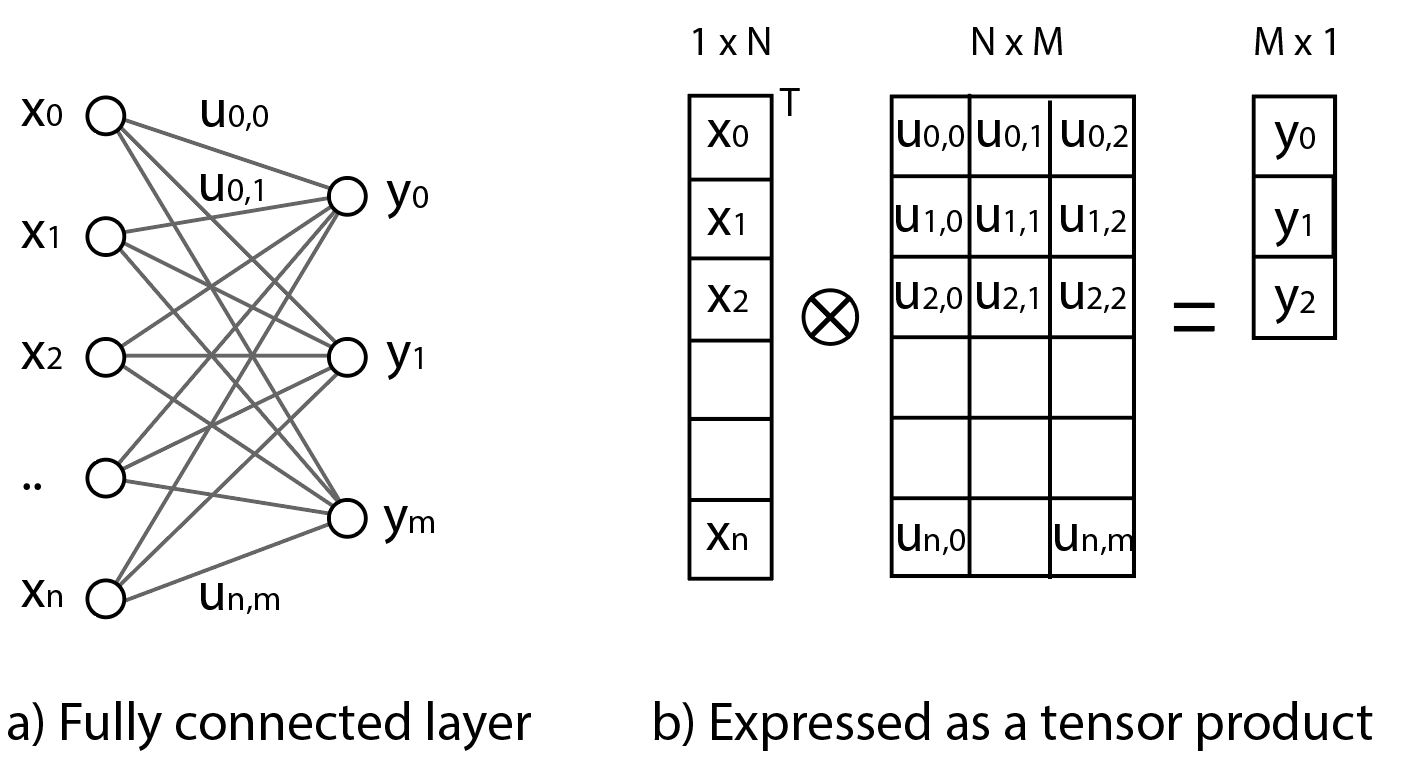
\includegraphics[width=0.4\textwidth]{images/Fully_connected_neural_network_and_it's_expression_as_a_tensor_product.jpg}
\end{wrapfigure}

A lot of operations in Machine Learning can be visualized and calculated in Matrix / Tensor Operations.

For example, a fully connected neural network! The same goes for most other operations in neural networks, including a large part of training specific operations, and is even more seen in Convolutional-NNs.

\textbf{Tensors} are n-dimensional arrays with n being called rank. A rank 0 tensor can also be called a scalar, a rank 1 tensor a vector and a rank 2 tensor a matrix for example.

\textbf{Quantization} is a technique used in ML to lower the resource need by lowering precision of weights and calculations. A commonly used format \textbf{bfloat16} has the same exponent range as 32 bit floats while having reduced floating point precision.


\section{Current Architecture}
Many current TPU Architectures have the same core at heart, namely a systolic array, of different sizes.

Examples of Chips utilizing Systolic Arrays are NVIDIA Tensor Cores, Google TPUs, AWS Inferentia2 \& Trainium and more..

\subsection{Systolic Arrays / Matrix Multiply Units}
\begin{wrapfigure}[7]{r}{0.3\textwidth}
    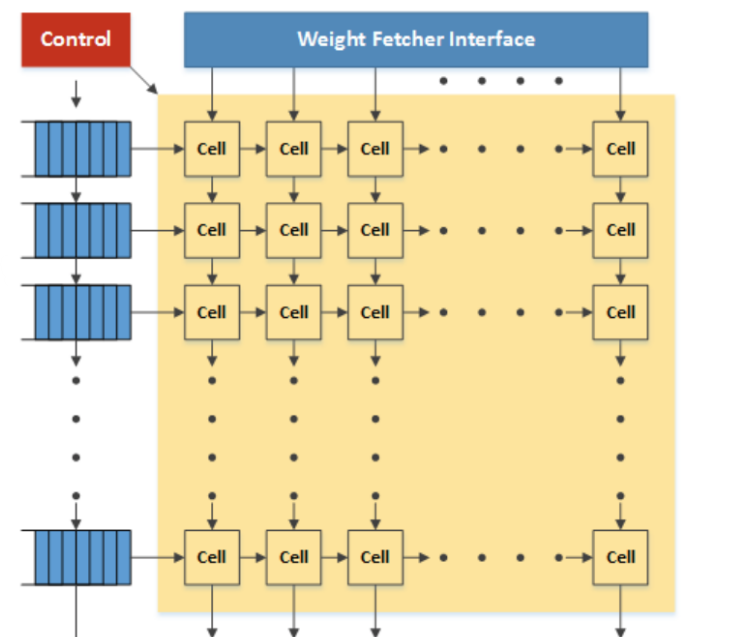
\includegraphics[width=0.3\textwidth]{images/MatrixMultiplayUnit.png}
\end{wrapfigure}

A \textbf{systolic array} is a matrix of processing pnits called cells. Each of these cells perform a calculation with the result then passed to the next cell. 

In TPUs Multiply-Accumulate Systolic Arrays find use to calculate the result of tensor products by streaming input vectors over a preloaded weight-matrix efficiently performing many calculations in one cycle without requiring memory writes.

\section{ML Platform Comparision}
\textbf{CPUs:}
Flexible and useful for small models and batch sizes with irregular implementation since general purpose. Not good for larger sized models or batch sizes.

\textbf{TPU:}
Very good for any operation utilizing tensor / matrix operations, so especially CNNs, and performing NN calculations on large batch sizes. Not good for general purpose calculations and for irregular models where flexibility is needed since application specific.

\textbf{GPU:}
Very good for almost any model but worse at Matrix Operations (not with Tensor Cores). Flexible and doesnt require standard implementations, easily programmable since general purpose.


\section{Compilation - TPU Example}
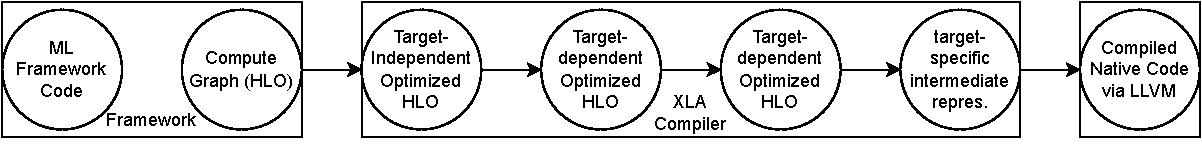
\includegraphics[width=1\textwidth]{images/Compile_Path.drawio.pdf}

\end{document}